\documentclass{article}
\usepackage{amsmath}  % Pacchetto per migliorare la resa matematica
\usepackage{amssymb}  % Per simboli matematici aggiuntivi
\usepackage{graphicx}
\usepackage[export]{adjustbox}
\usepackage{float}


\begin{document}

$G$ inizialmente contiene solo un nodo $\alpha$.  
Il primo albero $T_1$ viene inserito interamente e, per ogni nodo di $G$,  
si aggiunge ai nodi mappati il corrispettivo nodo di $T_1$.  
Infine, si aggiunge in $G$ un arco $(\alpha, \operatorname{root}(T_1))$.

Per inserire un generico albero $T_n$ successivo al primo,  
si effettua la seguente procedura partendo dalla radice $r$ di $T_n$.

\section*{insert\_tree}
Se esiste un nodo $x$ in $G$ tale che $\operatorname{label}(x) = \operatorname{label}(r) $
e $\operatorname{unique}(\operatorname{labels}(N_G^+(x))) = \operatorname{labels}(N_T^+(r))$ si aggiunge il nodo $r$ ai nodi mappati da $x$. Altrimenti, si aggiunge in $G$ un nuovo nodo $x$ con  
\(\operatorname{label}(x) = \operatorname{label}(r)\)  
e si aggiunge $r$ ai nodi mappati da $x$.

Ora sia $z$ il predecessore di $r$ in $T_n$ e sia $y$ il nodo in $G$ sul quale è mappato $z$.  
Se non esiste già, si aggiunge in $G$ un arco $(y, x)$.  
Se invece $r$ è la radice di $T_n$, si aggiunge in $G$ un arco $(\alpha, x)$.  
Infine, si esegue lo stesso procedimento per ognuno dei successori di $r$ in $T$.

\section*{insert\_tree\_rilassato}
si cerca un nodo $x$ in $G$ tale che $\operatorname{label}(x) = \operatorname{label}(r)$,  $\space \operatorname{labels}(N_T^+(r)) \subseteq \operatorname{labels}(N_G^+(x))$ e  che minimizza $\operatorname{length}(\operatorname{labels}(N_T^+(r)) - \operatorname{labels}(N_G^+(x)))$, se esiste si aggiunge il nodo $r$ ai nodi mappati da $x$, altrimenti si aggiunge in $G$ un nuovo nodo $x$ con $\operatorname{label}(x) = \operatorname{label}(r)$ e si aggiunge $r$ ai nodi mappati da $x$.

Ora sia $z$ il predecessore di $r$ in $T_n$ e sia $y$ il nodo in $G$ sul quale è mappato $z$. Se non esiste già, si aggiunge in $G$ un arco $(y, x)$. Se invece $r$ è la radice di $T_n$, si aggiunge in $G$ un arco $(\alpha, x)$. Infine, si esegue lo stesso procedimento per ognuno dei successori di $r$ in $T$.
\\ \\
Nella procedura di insert\_tree, se esiste, si troverà un solo nodo $x$ che rispetta le condizioni, invece nell'insert\_tree\_rilassato ad ogni passaggio potrebbero esserci più nodi tali che $\operatorname{label}(x) = \operatorname{label}(r)$ e $\space \operatorname{labels}(N_T^+(r)) \subseteq \operatorname{labels}(N_G^+(x))$, allora se ne prende uno che minimizza la differenza tra i figli del nodo $r$ e quelli del nodo $x$ ma questo potrebbe comunque non essere unico.
\clearpage
\section*{esempi}

\begin{figure}[H]
    \centering
    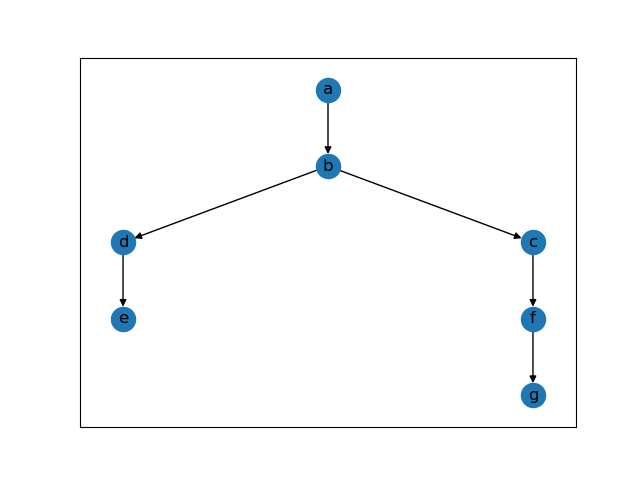
\includegraphics[width=0.4\textwidth]{Resources/T1.png}
    \hspace{0.5cm}
    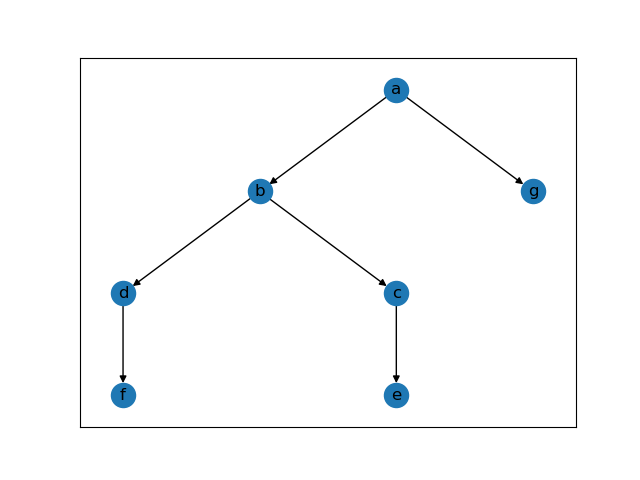
\includegraphics[width=0.4\textwidth]{Resources/T2.png}
    \hspace{0.5cm}
    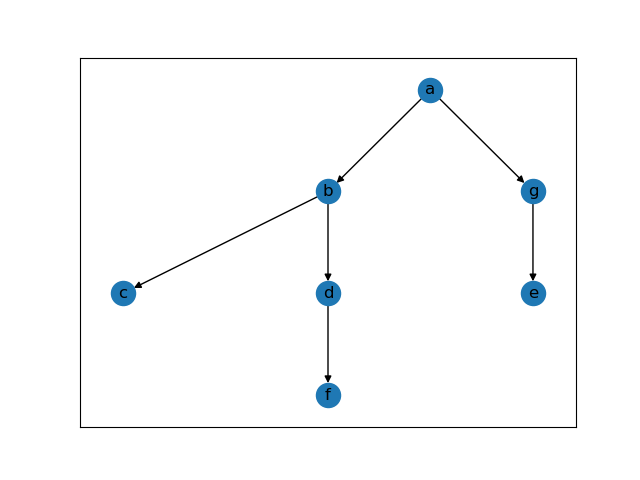
\includegraphics[width=0.4\textwidth]{Resources/T3.png}
    \hspace{0.5cm}
    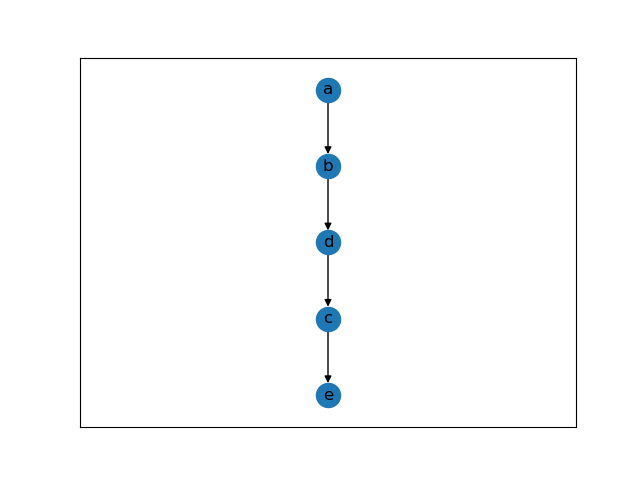
\includegraphics[width=0.4\textwidth]{Resources/T4.png}
    \caption{Alberi in input}
\end{figure}

\clearpage
\begin{figure}[H]
    \centering
    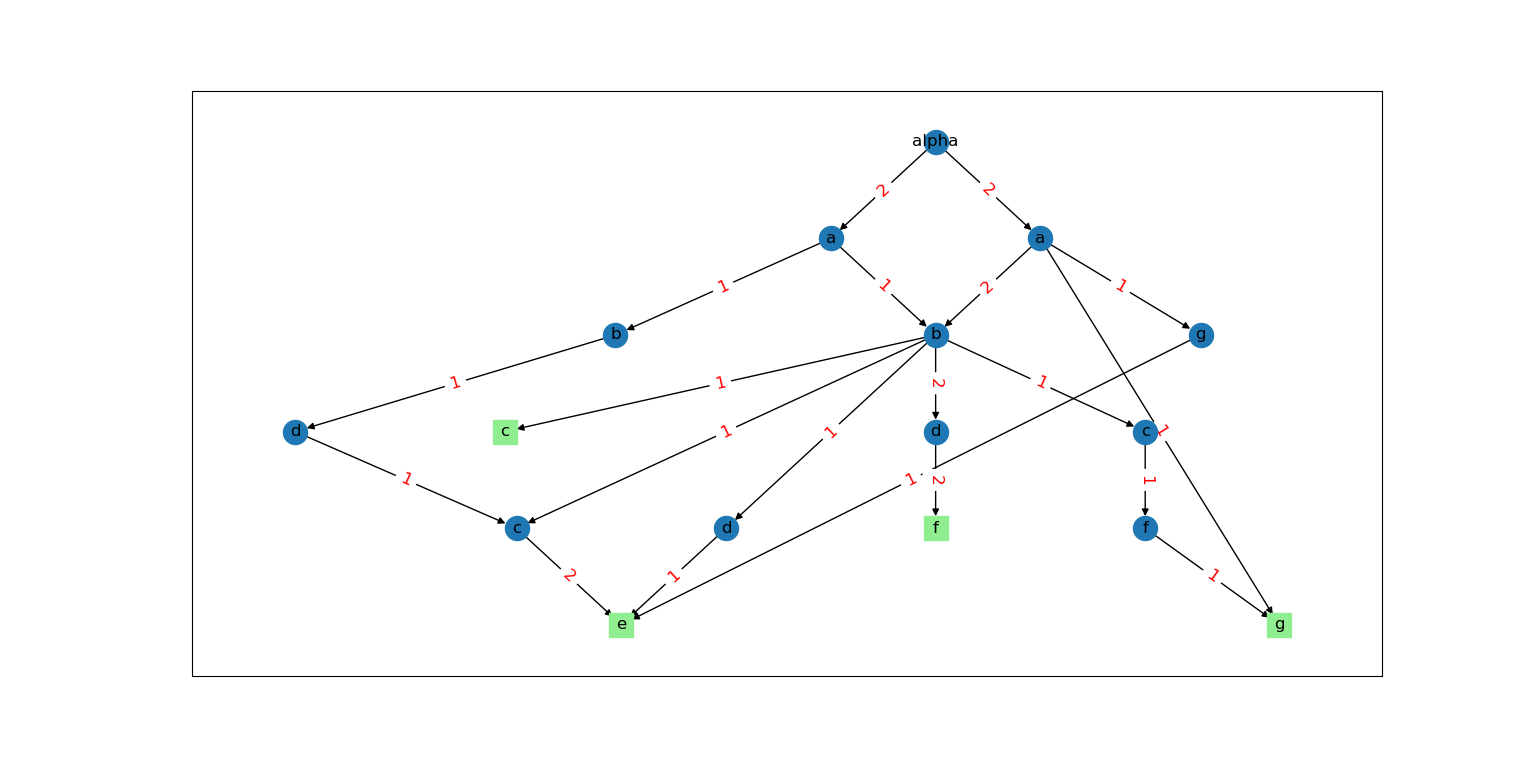
\includegraphics[max width=\linewidth, max height=0.9\textheight, keepaspectratio]{Resources/insert_tree.png}
    
    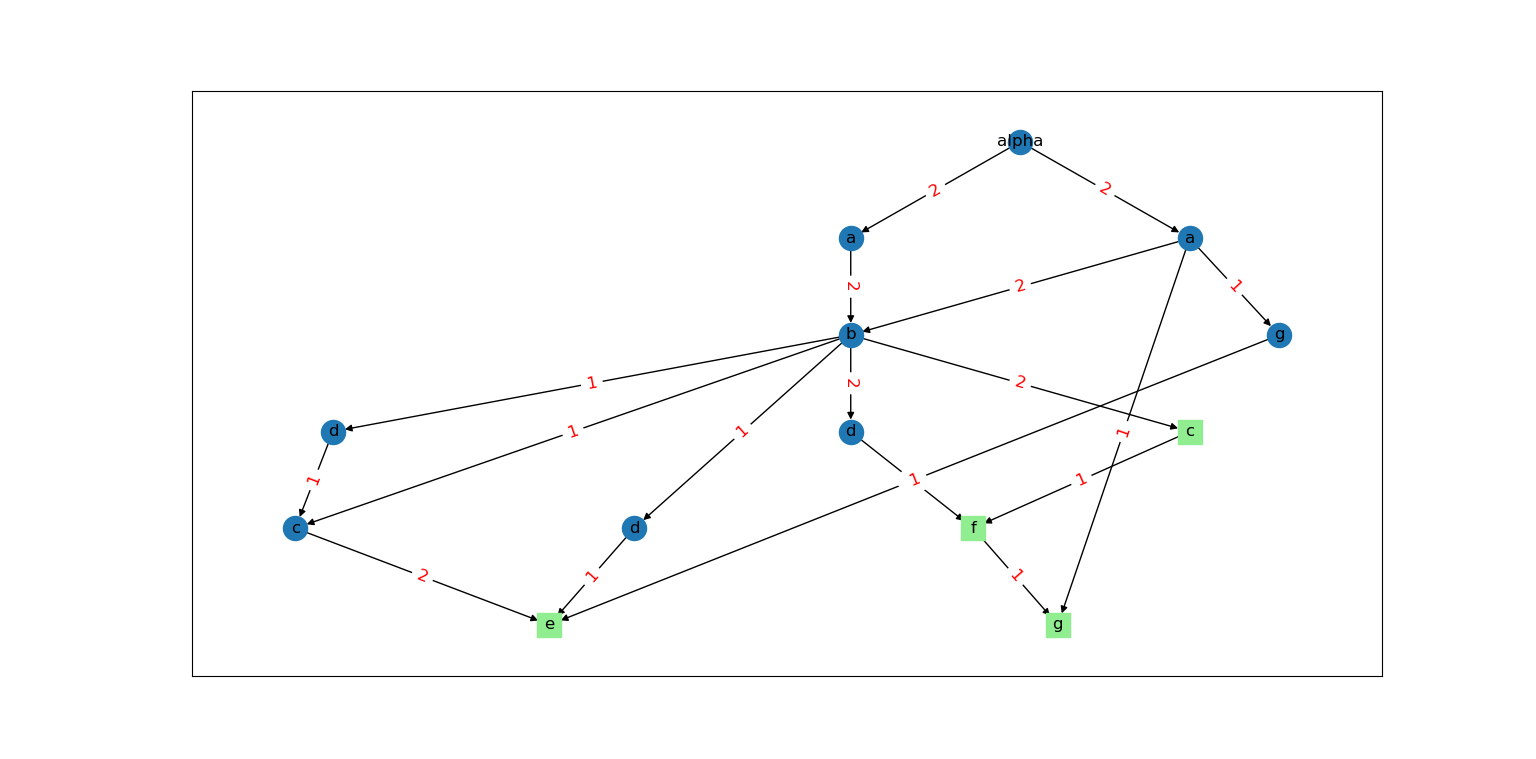
\includegraphics[max width=\linewidth, max height=0.9\textheight, keepaspectratio]{Resources/insert_tree_rilassato.png}
    \caption{Insert\_tree (sopra) e insert\_tree\_rilassato (sotto)}
    \label{fig:esempio}
\end{figure}

\begin{figure}[H]
    \centering
    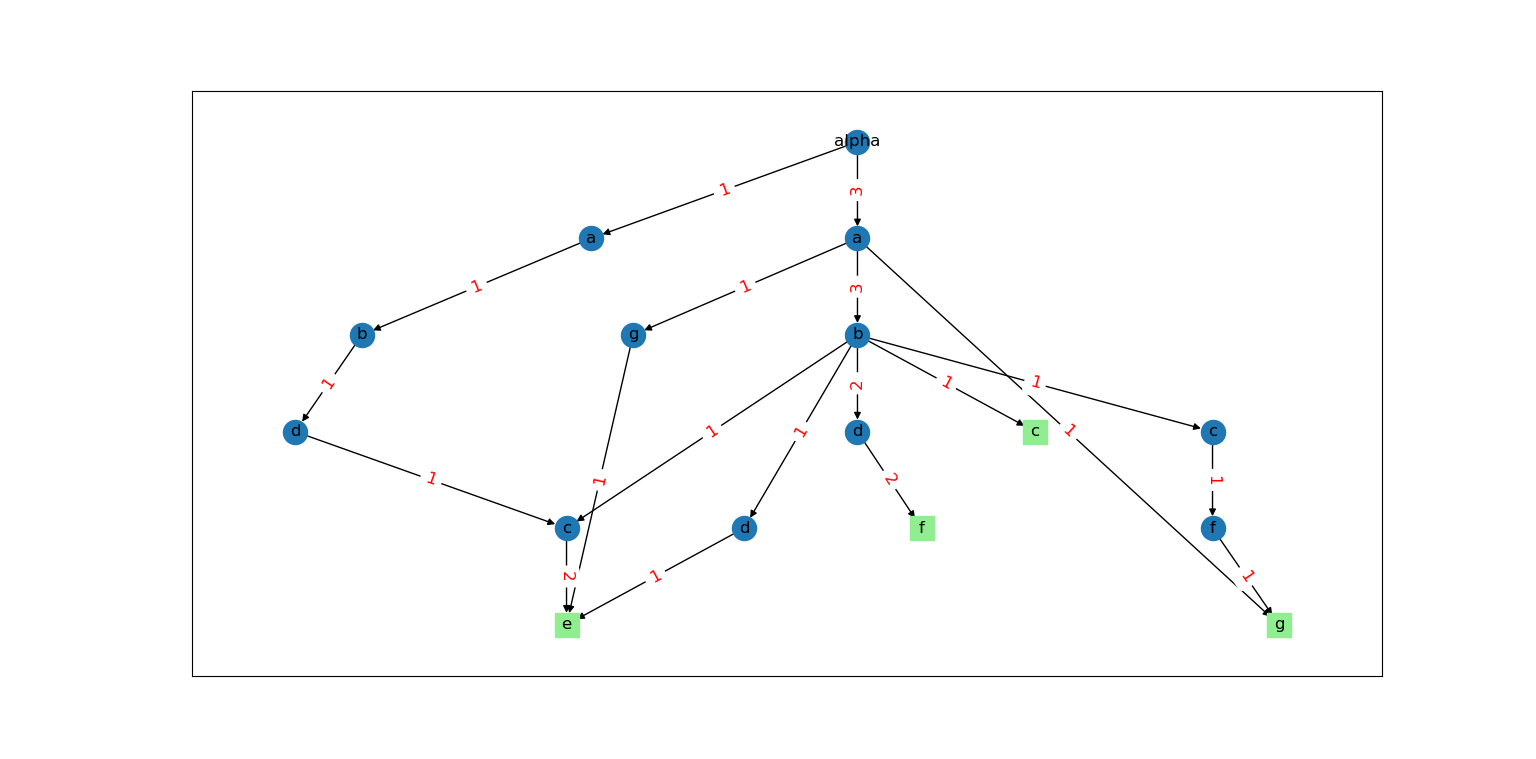
\includegraphics[max width=\linewidth, max height=0.9\textheight, keepaspectratio]{Resources/Uguaglianza+shrink.png}
    
    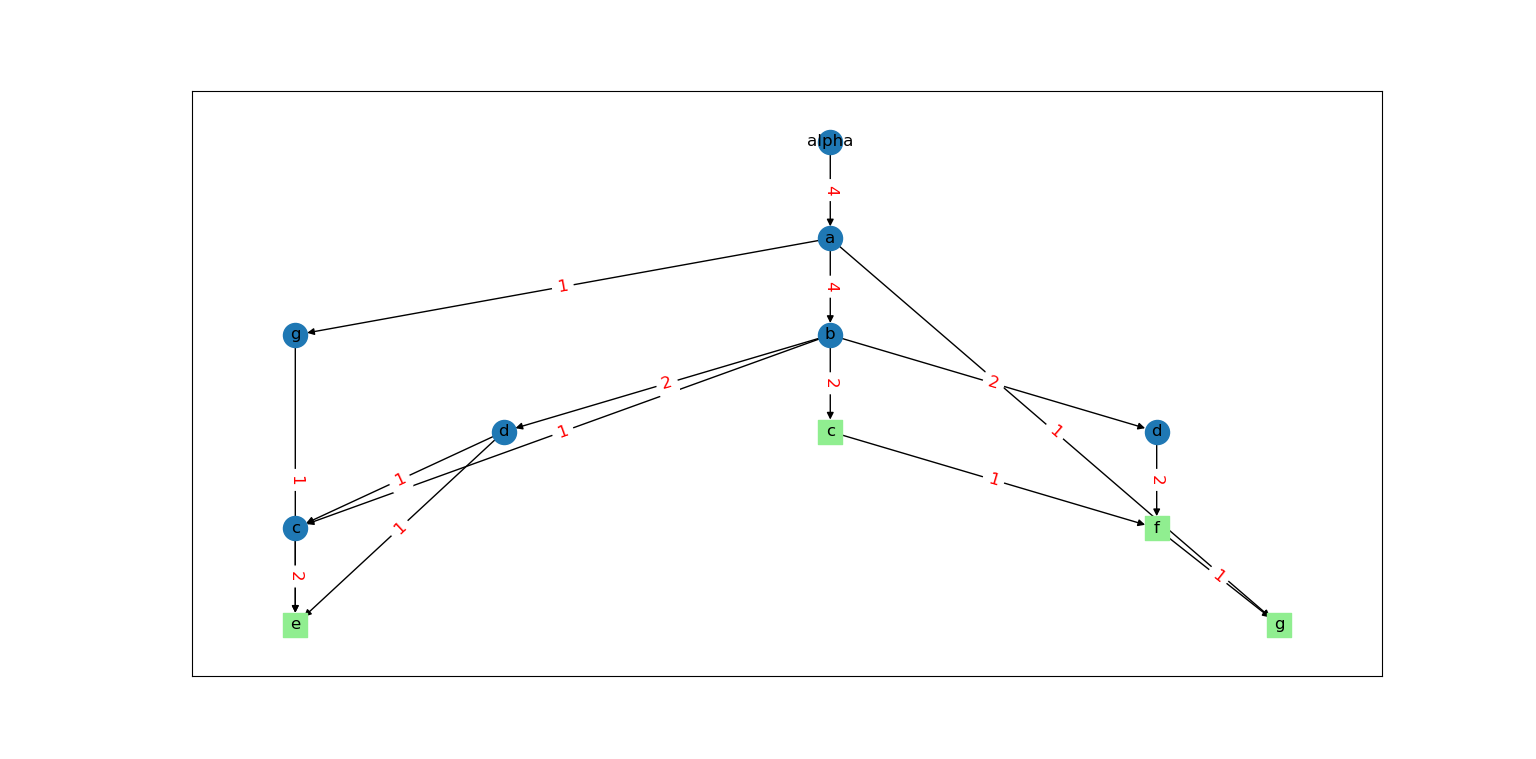
\includegraphics[max width=\linewidth, max height=0.9\textheight, keepaspectratio]{Resources/insert_tree_rilassato+shrink.png}
    \caption{Insert\_tree + shrink (sopra) e insert\_tree\_rilassato + shrink (sotto)}
    \label{fig:esempio2}
\end{figure}

\begin{figure}[H]
    \centering
    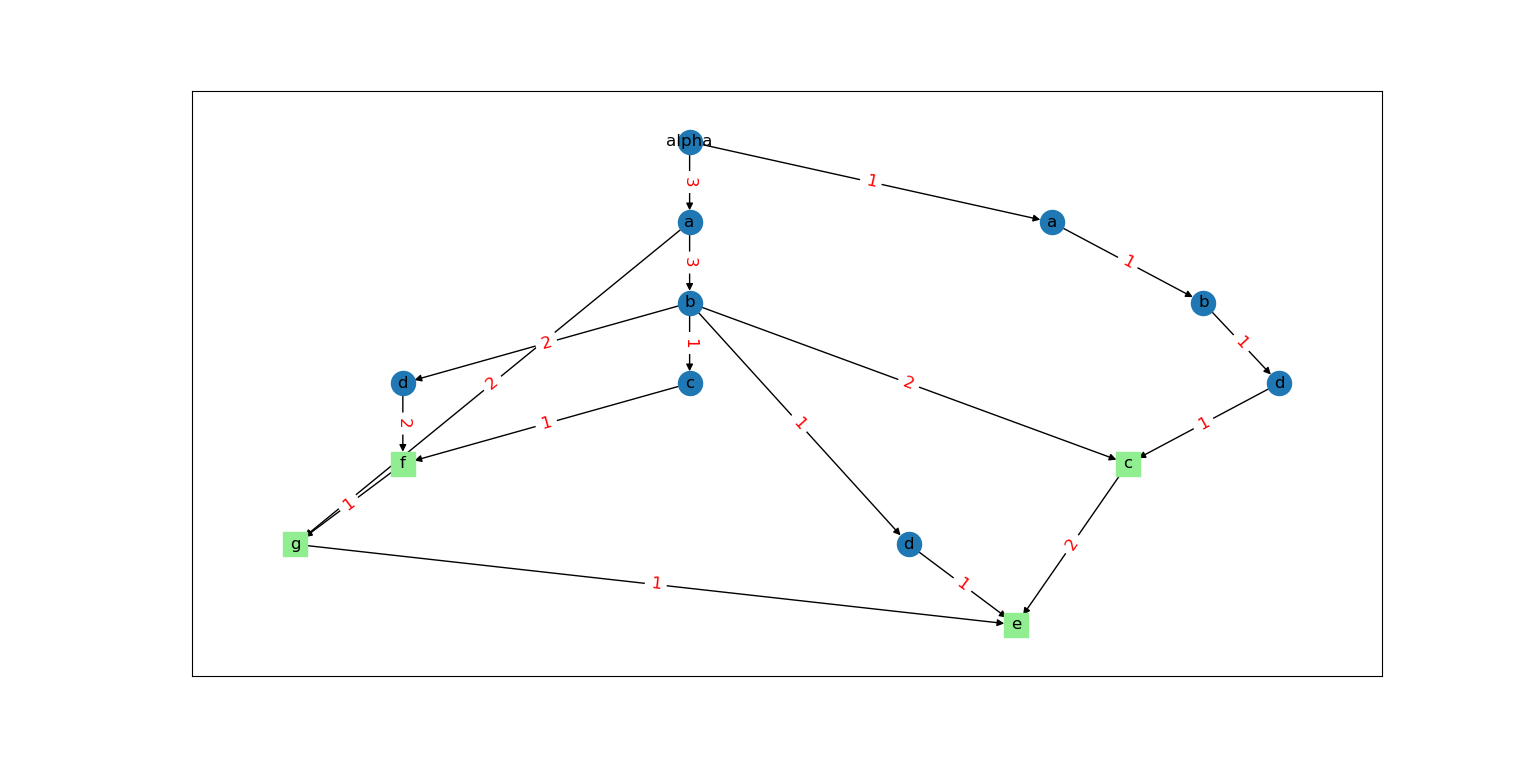
\includegraphics[max width=\linewidth, max height=0.9\textheight, keepaspectratio]{Resources/Uguaglianza+incorporate.png}
    
    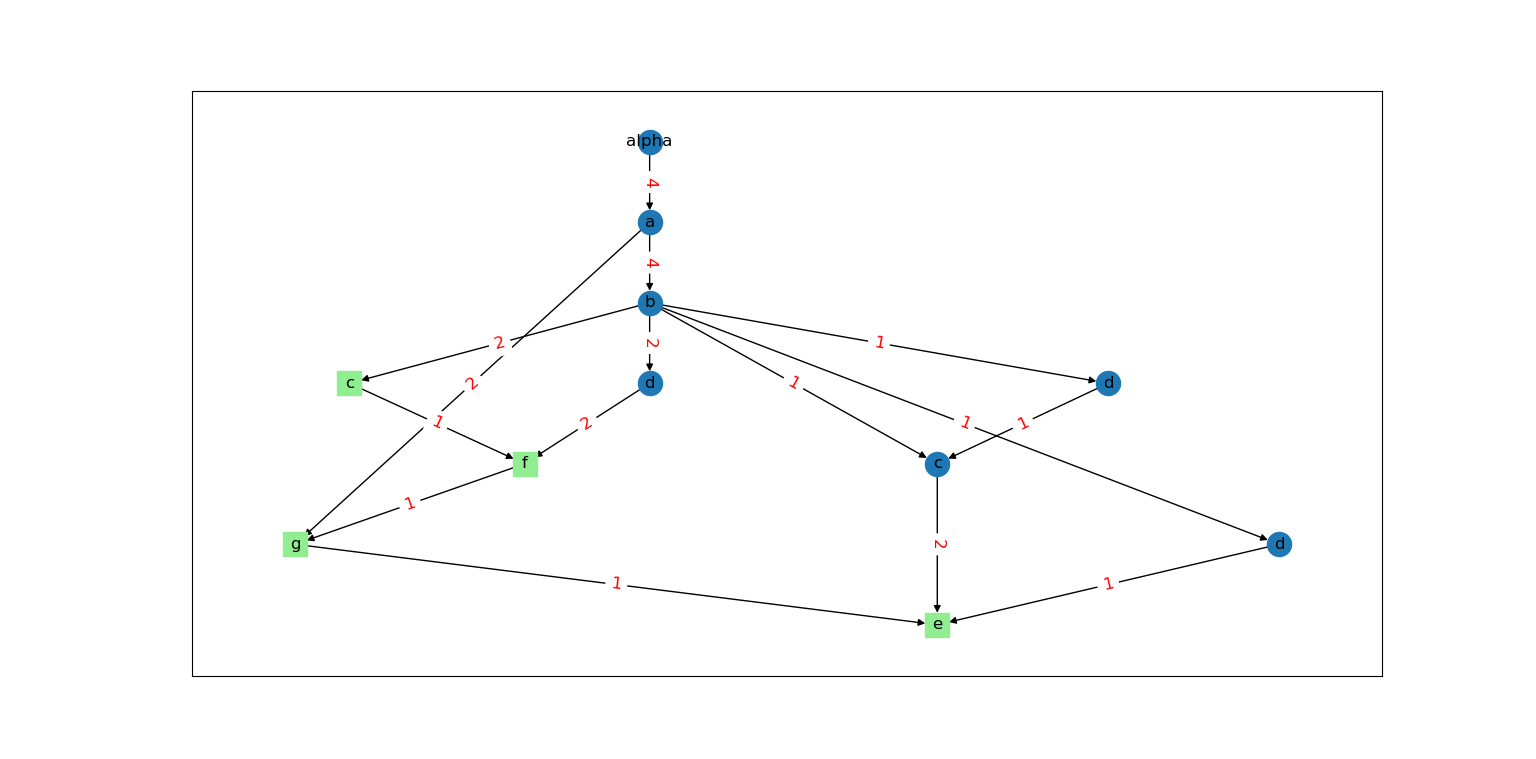
\includegraphics[max width=\linewidth, max height=0.9\textheight, keepaspectratio]{Resources/insert_tree_rilassato+incorporate.png}
    \caption{Insert\_tree + incorporate (sopra) e insert\_tree\_rilassato + incorporate (sotto)}
    \label{fig:esempio3}
\end{figure}

\begin{figure}[H]
    \centering
    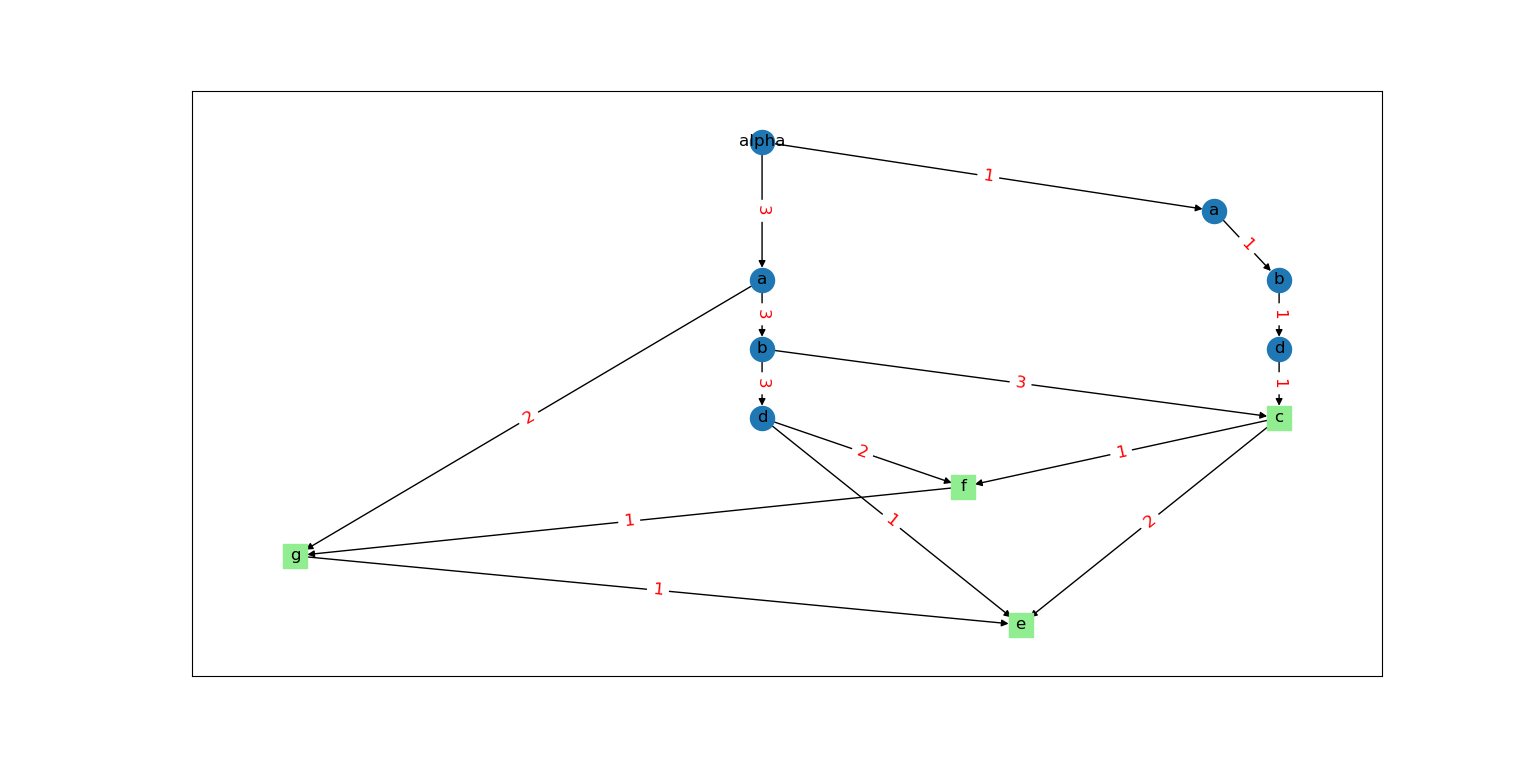
\includegraphics[max width=\linewidth, max height=0.9\textheight, keepaspectratio]{Resources/Uguaglianza+shrink+incorporate.png}
    
    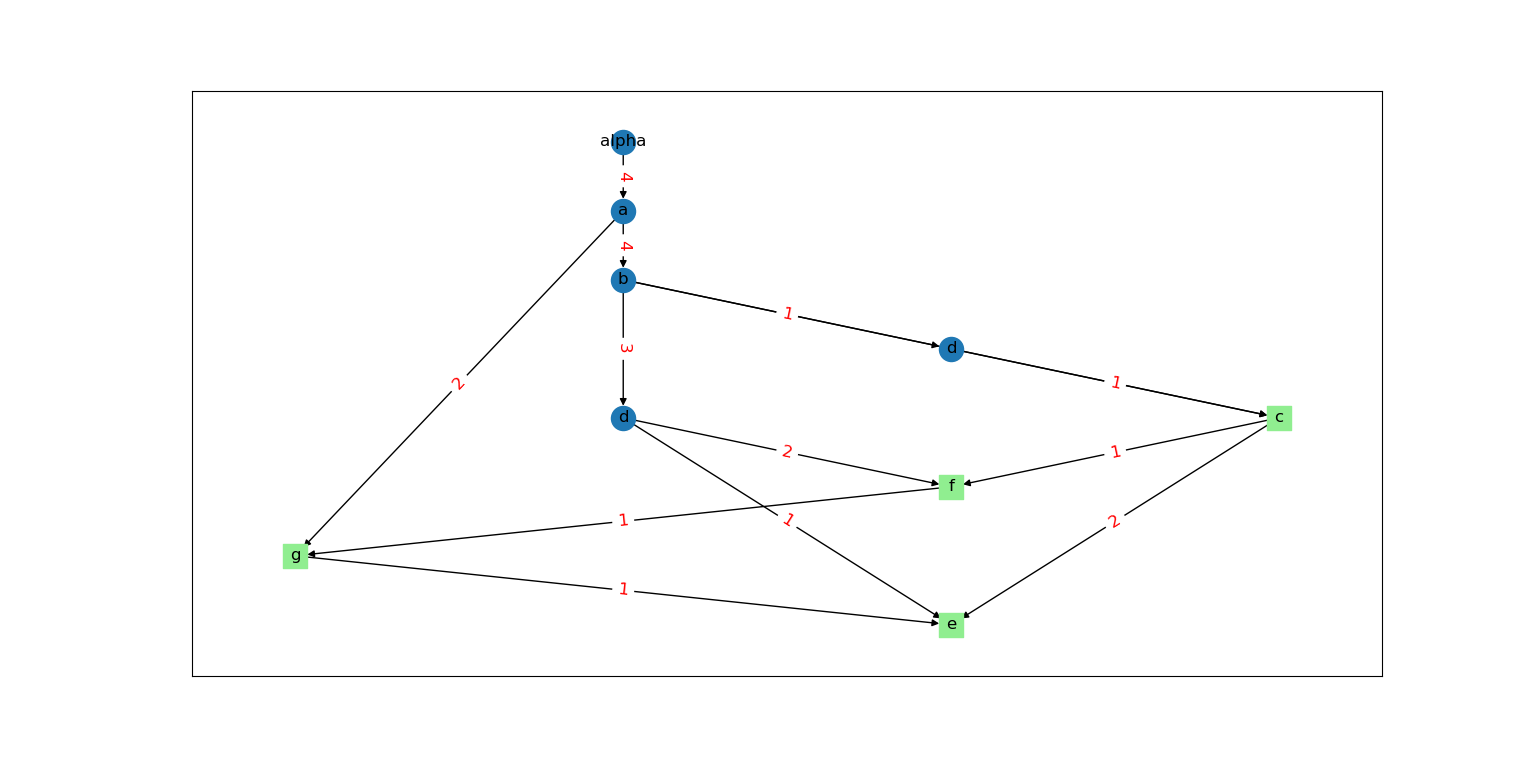
\includegraphics[max width=\linewidth, max height=0.9\textheight, keepaspectratio]{Resources/insert_tree_rilassato+shrink+incorporate.png}
    \caption{Insert\_tree + shrink + incorporate (sopra) e insert\_tree\_rilassato + shrink + incorporate (sotto)}
    \label{fig:esempio4}
\end{figure}

\end{document}
